\section{Probabilités discrètes}

\begin{definition}[Expérience Aléatoire (\textit{random experiment})]
  Une \textbf{expérience aléatoire} est une expérience dont le résultat n'est pas
  prévisible.
\end{definition}
Formellement, une telle expérience se décrit comme un élément $\omega$ pris
dans un ensemble $\Omega$ de résultats possibles, appelé l'\textbf{univers}
(\textit{sample space}).

Lorsque l'univers $\Omega$ est un ensemble au plus dénombrable, on peut définir
une théorie de la probabilites élémentaire, qui ne nécessite pas la théorie de
la mesure.  Chaque événement peut être affecté d'une probabilité, et les
probabilités des événements sont reliées par les axiomes de Kolmogorov. Cette
théorie est appelée la théorie des probabilités discrètes,

\subsection{Espace de probabilité discret}

On se restreint au cas où l'univers $\Omega$ est un ensemble au plus
dénombrable. On note $\mathcal{P}(\Omega)$ l'\textbf{ensemble des parties} de
$\Omega$.

\begin{definition}[Événement]
  On appelle \textbf{événement} (\textit{event}) tout sous-ensemble de $\Omega$.
\end{definition}

On dit que l'événement $A$ est réalisé si $\omega \in A$.\\

The whole vocabulary of set operations carries a probabilistic reading. Comme
les événements sont des ensembles, on obtient pour tous événements $A$ et $B$ :

\begin{itemize}
  \item $A^{c} = \Omega \setminus A$ : l'événement ``non $A$'' ;
  \item $A \intersect B$ : l'événement ``$A$ et $B$'' ; $A \union B$ :
    l'événement ``$A$ ou $B$'' ;
  \item $A \subr B$ : la propriété ``$A$ implique $B$'' ;
  \item $A \intersect B = \emptyset$ : la propriété ``$A$ et $B$ incompatibles''.
\end{itemize}

Par ailleurs, les ensembles $\emptyset$ et $\Omega$ définissent des événements,
respectivement impossible et certain: the two extreme cases, the
\textbf{événement impossible} (\textit{impossible event}) and the
\textbf{événement certain} (\textit{certain event}).

\begin{definition}[Mesure de probabilité]
  On appelle \textbf{mesure de probabilité} (\textit{probability measure}) sur un
  ensemble au plus dénombrable $\Omega$ une application
  $\prob : \mathcal{P}(\Omega) \to [0,1]$ qui satisfait les deux propriétés
  suivantes :
  \begin{itemize}
    \item $\prob(\Omega) = 1$ ;
    \item pour toute famille au plus dénombrable d'événements deux-à-deux
      disjoints $(A_{i})_{i \in I}$,
      \[ \prob\left( \bigcup_{i \in I} A_{i} \right)
           = \sum_{i \in I} \prob(A_{i}). \]
  \end{itemize}
  On appelle la seconde propriété l'axiome de
  \textbf{$\sigma$-additivité} (\textit{$\sigma$-additivity}).
\end{definition}

The two hypotheses on the family matter and are often quoted loosely. The family
must be at most countable --- $\sigma$-additivité says nothing about an
uncountable union --- and the événements must be \emph{pairwise} disjoint, not
merely have empty total intersection.

\begin{remark}
  Une mesure de probabilité sur un espace discret est entièrement caractérisée
  par ses valeurs prises sur les singletons, puisque pour tout $A \subr \Omega$,
  \[ \prob(A) = \sum_{\omega \in A} \prob(\{\omega\}). \]
  This is the one structural simplification the discrete setting buys, and it is
  exactly what fails in the general case: on $\reals$ every singleton has
  probability $0$, yet the mesure is not zero.
\end{remark}

\begin{prop}
  Soit $\prob$ une mesure de probabilité sur $\Omega$. Pour tous
  $A, B \subr \Omega$,
  \begin{enumerate}
    \item $\prob(\emptyset) = 0$;
    \item $\prob(A^{c}) = 1 - \prob(A)$;
    \item $\prob(A \union B) = \prob(A) + \prob(B) - \prob(A \intersect B)$;
    \item si $A \subr B$, alors $\prob(A) \le \prob(B)$.
  \end{enumerate}
\end{prop}

\textbf{Suite d'événements.} Une suite d'événements $(A_{n})_{n \ge 1}$ est dite
\emph{croissante} si $A_{n} \subr A_{n+1}$ pour tout $n$ ; sa limite est alors
$A = \union_{n} A_{n}$, ce que l'on notera $A_{n} \uparrow A$. De même, une suite
d'événements est dite \emph{décroissante} si $A_{n+1} \subr A_{n}$ pour tout
$n$ ; sa limite est $A = \intersect_{n} A_{n}$, ce que l'on notera
$A_{n} \downarrow A$.

\begin{prop}
  Soit $\prob$ une mesure de probabilité sur $\Omega$ et $(A_{n})_{n \ge 1}$ une
  suite d'événements.
  \begin{enumerate}
    \item Si $A_{n} \uparrow A$, alors $\prob(A) = \lim_{n} \uparrow \prob(A_{n})$.
    \item Si $A_{n} \downarrow A$, alors
      $\prob(A) = \lim_{n} \downarrow \prob(A_{n})$.
    \item On a la \textbf{borne de l'union} (\textit{union bound}) :
      \[ \prob\left( \bigcup_{n \ge 1} A_{n} \right)
           \le \sum_{n \ge 1} \prob(A_{n}). \]
  \end{enumerate}
\end{prop}

\begin{remark}
  These are the discrete shadow of convergence monotone. The increasing case is
  $\sigma$-additivité after disjointification --- set $B_{1} = A_{1}$ and
  $B_{n} = A_{n} \setminus A_{n-1}$. For the decreasing case, by
  complementation, la preuve découle de la propriété précédente, en remarquant
  que $A_{n} \downarrow A$ implique $A_{n}^{c} \uparrow A^{c}$.
  The borne de l'union is finite subadditivity iterated, then passed to the
  limit. All three reappear in chapter 2 for a general mesure, where the
  decreasing case acquires a finiteness hypothesis that is automatic here.
\end{remark}

\subsection{Indépendance}

\begin{definition}[Indépendance (\textit{independence})]
  Deux événements $A$, $B$ sont dits \textbf{indépendants}, ce que l'on note
  $A \indep B$, si
  \[ \prob(A \intersect B) = \prob(A)\prob(B). \]
\end{definition}

La notion d'indépendance est donc liée à la mesure de probabilité: it is not a
property of the sets, but of the sets \emph{together with} the mesure. The same
two subsets of the same $\Omega$ can be independent for one mesure and dependent
for another, and this is why conditioning --- which replaces $\prob$ by
$\prob(\cdot \mid C)$ --- can destroy or create it.

\begin{prop}
  Il y a équivalence entre $A \indep B$, $A \indep B^{c}$, $A^{c} \indep B$ et
  $A^{c} \indep B^{c}$.
\end{prop}

\begin{prop}
  Un événement $A$ tel que $\prob(A) = 0$ ou $\prob(A) = 1$ est indépendant de
  tout autre événement.
\end{prop}

\begin{definition}[Événements indépendants (\textit{independent events})]
  Les événements d'une famille $(A_{i})_{i \in I}$ sont dits
  \textbf{indépendants} si pour tout sous-ensemble \emph{fini} $J \subr I$,
  \[ \prob\left( \bigcap_{i \in J} A_{i} \right)
       = \prod_{i \in J} \prob(A_{i}). \]
\end{definition}

The quantifier over all finite subsets is the whole content of the definition.
Checking the single identity $\prob(\intersect_{i \in I} A_{i}) = \prod_{i \in I}
\prob(A_{i})$, or checking it only on pairs, is strictly weaker.

\begin{example}[Pairwise indépendance is not indépendance]
  Throw a die twice, and consider the three événements ``le premier lancer est
  pair'', ``le second lancer est pair'' and ``la somme des deux lancers est
  paire''. Each has probability $\tfrac{1}{2}$, and any two of them are
  independent: knowing the parity of one throw says nothing about the parity of
  the other, and the parity of the sum is equally likely either way given one
  throw. But the three are not independent, because the third événement is the
  événement that the first two \emph{agree}: the intersection of all three has
  probability $\tfrac{1}{4}$, not $\tfrac{1}{8}$. Taken two at a time, though,
  les événements ``le premier lancer est pair'' et ``la somme des deux lancers
  est paire'' sont indépendants --- an identity between numbers, not a fact
  about the experiment. Ainsi, les événements ``le premier lancer est impair'' et
  ``la somme des deux lancers est impaire'' sont également indépendants, by the
  proposition above.
\end{example}

\subsection{Conditionnement}

\begin{definition}[Probabilité conditionnelle]
  Pour tous événements $A$, $B$ tels que $\prob(B) > 0$, on définit la
  \textbf{probabilité conditionnelle} (\textit{conditional probability}) de $A$
  sachant $B$ par :
  \[ \prob(A \mid B) = \frac{\prob(A \intersect B)}{\prob(B)}. \]
\end{definition}

The hypothesis $\prob(B) > 0$ is not cosmetic: the whole of chapter 5 exists to
give a meaning to conditioning on an événement of probability zero, which is the
generic situation once densités appear. In the discrete setting it can simply be
required.

\begin{prop}
  Pour tout événement $B$ tel que $\prob(B) > 0$, l'application
  $A \mapsto \prob(A \mid B)$ est une mesure de probabilité sur $\Omega$.
\end{prop}

Everything already proved therefore applies verbatim to $\prob(\cdot \mid B)$:
complementation, inclusion--exclusion, monotone limits, the borne de l'union.
Tout se passe comme si l'univers, initialement $\Omega$, était réduit à $B$ ---
and renormalised.

\begin{prop}
  Deux événements $A$ et $B$ sont indépendants si et seulement si
  $\prob(B) = 0$ ou $\prob(A \mid B) = \prob(A)$.
\end{prop}

\begin{prop}[Formule de Bayes (\textit{Bayes' formula})]
  Soit $A$, $B$ deux événements tels que $\prob(A) > 0$ et $\prob(B) > 0$. Alors,
  \[ \prob(A \mid B) = \frac{\prob(B \mid A)\,\prob(A)}{\prob(B)}. \]
\end{prop}

Both positivity hypotheses are needed: $\prob(B) > 0$ for the left-hand side to
exist, $\prob(A) > 0$ for the probabilité conditionnelle on the right. La
formule de Bayes permet de changer l'ordre du conditionnement. La preuve est
immédiate: $\prob(A \intersect B)$ can be factored two ways.

\begin{definition}[Indépendance conditionnelle (\textit{conditional independence})]
  Soit $C$ un événement tel que $\prob(C) > 0$. Deux événements $A$, $B$ sont
  dits \textbf{indépendants conditionnellement à} $C$, ce que l'on note
  $A \indep B \mid C$, s'ils sont indépendants pour la probabilité
  conditionnelle $\prob(\cdot \mid C)$ :
  \[ \prob(A \intersect B \mid C) = \prob(A \mid C)\,\prob(B \mid C). \]
\end{definition}

\begin{prop}
  Soit $C$ un événement tel que $\prob(C) > 0$. Deux événements $A$ et $B$ sont
  indépendants conditionnellement à $C$ si et seulement si $\prob(B \mid C) = 0$
  ou $\prob(A \mid B \intersect C) = \prob(A \mid C)$.
\end{prop}

\begin{example}[Conditioning destroys indépendance]
  On lance un dé deux fois. Les événements ``le premier lancer est pair'' et
  ``le second lancer est pair'' sont indépendants, mais \emph{pas}
  conditionnellement à l'événement ``la somme des deux lancers est paire''.
  Given that the sum is even, the two throws have the same parity, so knowing
  that the first is even forces the second to be. Indépendance conditionnelle is
  neither implied by, nor implies, indépendance.
\end{example}

\begin{prop}[Formule des probabilités composées (\textit{chain rule})]
  Pour tous événements $A_{1}, \dots, A_{n}$ tels que
  $\prob(A_{1} \intersect \dots \intersect A_{n}) > 0$,
  \[ \prob(A_{1} \intersect \dots \intersect A_{n})
       = \prob(A_{1}) \prob(A_{2} \mid A_{1}) \cdots
         \prob(A_{n} \mid A_{1} \intersect \dots \intersect A_{n-1}). \]
\end{prop}

The positivity hypothesis is on the \emph{full} intersection. It is what makes
every conditioning on the right-hand side legitimate at once, since each
conditioning événement contains $A_{1} \intersect \dots \intersect A_{n}$ and
therefore has positive probability too.

\begin{prop}[Formule des probabilités totales (\textit{law of total probability})]
  Pour toute famille d'événements $(B_{i})_{i \in I}$ formant une partition de
  $\Omega$, avec $\prob(B_{i}) > 0$ pour tout $i \in I$,
  \[ \prob(A) = \sum_{i \in I} \prob(B_{i}) \prob(A \mid B_{i}). \]
\end{prop}

Il suffit d'écrire $A = \union_{i \in I} (A \intersect B_{i})$: the union is
disjoint, so $\sigma$-additivité applies; the family must therefore be at most
countable, like everything else here. The two formulas are usually used
together: the formule des probabilités totales supplies the denominator
$\prob(B)$ that the formule de Bayes needs.

\begin{figure}[h!]
  \centering
  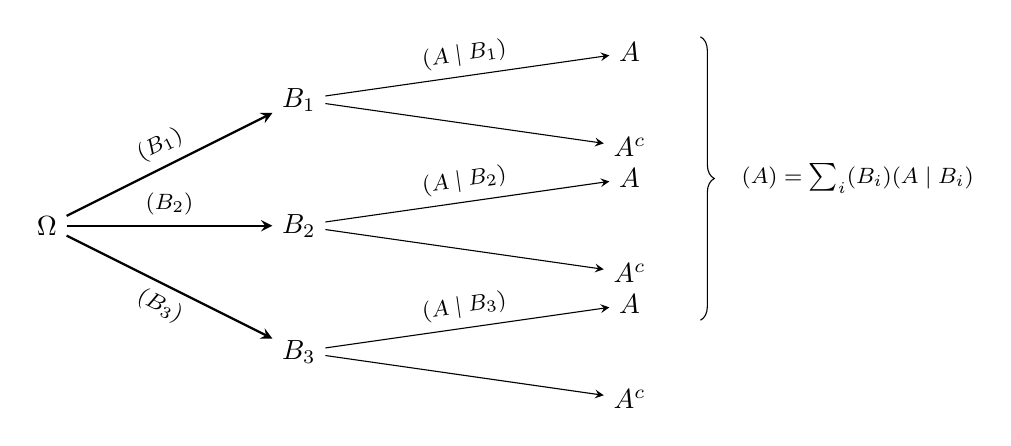
\begin{tikzpicture}[>=stealth, scale=1.0]
    \node (root) at (0,0) {$\Omega$};
    \node (b1) at (3.2,1.6) {$B_{1}$}; \node (b2) at (3.2,0.0) {$B_{2}$};
    \node (b3) at (3.2,-1.6) {$B_{3}$};
    \node (a1) at (7.4,2.2) {$A$};  \node (n1) at (7.4,1.0) {$A^{c}$};
    \node (a2) at (7.4,0.6) {$A$};  \node (n2) at (7.4,-0.6) {$A^{c}$};
    \node (a3) at (7.4,-1.0) {$A$}; \node (n3) at (7.4,-2.2) {$A^{c}$};
    \draw[->,thick] (root) -- (b1) node[midway,above,sloped] {\footnotesize $\prob(B_{1})$};
    \draw[->,thick] (root) -- (b2) node[midway,above] {\footnotesize $\prob(B_{2})$};
    \draw[->,thick] (root) -- (b3) node[midway,below,sloped] {\footnotesize $\prob(B_{3})$};
    \draw[->] (b1) -- (a1) node[midway,above,sloped] {\footnotesize $\prob(A \mid B_{1})$};
    \draw[->] (b2) -- (a2) node[midway,above,sloped] {\footnotesize $\prob(A \mid B_{2})$};
    \draw[->] (b3) -- (a3) node[midway,above,sloped] {\footnotesize $\prob(A \mid B_{3})$};
    \draw[->] (b1) -- (n1); \draw[->] (b2) -- (n2); \draw[->] (b3) -- (n3);
    \draw[decorate,decoration={brace,amplitude=5pt}] (8.3,2.4) -- (8.3,-1.2);
    \node[right] at (8.7,0.6)
      {\footnotesize $\prob(A) = \sum_{i} \prob(B_{i})\prob(A \mid B_{i})$};
  \end{tikzpicture}
\end{figure}

Reading the tree left to right gives the formule des probabilités totales: each
path to an $A$ leaf contributes the product of the probabilities along it, and
the paths are disjoint. Reading it right to left --- which branch did we come
down, given that we landed on $A$? --- is the formule de Bayes.

\begin{example}[A screening test with a small prevalence]
  On dispose d'un test pour une certaine maladie. Ce test n'est pas parfait :
  $1\%$ des individus sains sont positifs au test et $2\%$ des individus malades
  sont négatifs au test. On suppose que la maladie touche $1\%$ de la population.
  Quelle est la probabilité qu'un individu positif au test soit effectivement
  malade ?\\

  Soit $X$ l'état de l'individu et $Y$ le résultat du test. Par la formule de
  Bayes,
  \[ \prob(X = +\mid Y = +)
       = \frac{\prob(X=+)}{\prob(Y=+)}\, \prob(Y = + \mid X = +), \]
  on a $\prob(X=+) = 1\%$ et $\prob(Y=+\mid X=+) = 1 - 2\% = 98\%$. Il reste à
  appliquer la formule des probabilités totales --- for the denominator, with
  the partition $\{X=+\}, \{X=-\}$ --- pour obtenir :
  \[ \prob(Y=+) = 99\% \times 1\% + 1\% \times 98\%. \]
  Et donc
  \[ \prob(X = +\mid Y=+)
       = \frac{1\% \times 98\%}{99\% \times 1\% + 1\% \times 98\%}
       \simeq 50\%. \]
  A test that is $98\%$ and $99\%$ accurate identifies the ill barely better than
  a coin, because the prevalence and the false-positive rate are the same order
  of magnitude. The lesson is that $\prob(X \mid Y)$ and $\prob(Y \mid X)$ are
  different numbers, and that the prior is what separates them.
\end{example}

\begin{example}[Two walkers on a heptagon, as a conditioning computation]
  Two walkers move on the vertices of a heptagon, numbered $0$ to $6$. At each
  time $n$ each walker moves independently and uniformly to one of the two
  neighbouring vertices, so that with $X_{n}$ and $Y_{n}$ their positions,
  \[ \prob(X_{n+1} = X_{n} + 1 \bmod 7)
       = \prob(X_{n+1} = X_{n} - 1 \bmod 7) = \tfrac{1}{2}, \]
  and likewise for $Y_{n}$. Let $L_{n}$ be the length of the shortest path
  between the two walkers,
  \[ L_{n} = \min(X_{n} - Y_{n} \bmod 7,\ Y_{n} - X_{n} \bmod 7)
       \in \{0,1,2,3\}. \]
  Write $D_{n} = X_{n} - Y_{n} \bmod 7$, so that $L_{n} = \min(D_{n}, 7-D_{n})$.
  Each walker moves by $\pm 1$, so $D$ changes by $+2$, $0$ or $-2$ with
  probabilities $\tfrac14, \tfrac12, \tfrac14$. From $D=0$ the gap becomes $2$ or
  $5$, both at distance $2$; from $D=1$ it becomes $3$ or $6$, at distances $3$
  and $1$; from $D=2$ it becomes $4$ or $0$, at distances $3$ and $0$; from $D=3$
  it becomes $5$ or $1$, at distances $2$ and $1$. The loi of $L_{n+1}$
  therefore depends on the past only through $L_{n}$, which is the Markov
  property, and the transition probabilities
  $\prob(L_{n+1} = \ell' \mid L_{n} = \ell)$ are collected in the graph below.\\

  \begin{center}
  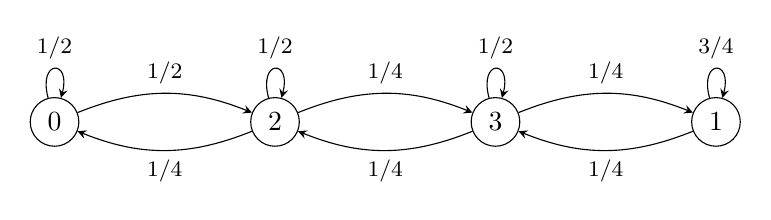
\begin{tikzpicture}[>=stealth, scale=1.0]
    \node[draw,circle] (s0) at (0,0) {$0$};   \node[draw,circle] (s2) at (2.8,0) {$2$};
    \node[draw,circle] (s3) at (5.6,0) {$3$}; \node[draw,circle] (s1) at (8.4,0) {$1$};
    \draw[->] (s0) to[bend left=22] node[above]{\footnotesize $1/2$} (s2);
    \draw[->] (s2) to[bend left=22] node[below]{\footnotesize $1/4$} (s0);
    \draw[->] (s2) to[bend left=22] node[above]{\footnotesize $1/4$} (s3);
    \draw[->] (s3) to[bend left=22] node[below]{\footnotesize $1/4$} (s2);
    \draw[->] (s3) to[bend left=22] node[above]{\footnotesize $1/4$} (s1);
    \draw[->] (s1) to[bend left=22] node[below]{\footnotesize $1/4$} (s3);
    \draw[->] (s0) to[loop above] node{\footnotesize $1/2$} (s0);
    \draw[->] (s2) to[loop above] node{\footnotesize $1/2$} (s2);
    \draw[->] (s3) to[loop above] node{\footnotesize $1/2$} (s3);
    \draw[->] (s1) to[loop above] node{\footnotesize $3/4$} (s1);
  \end{tikzpicture}
  \end{center}

  The graph is connected in both directions, so the chain is irreducible, and
  every state carries a self-loop, so it is aperiodic; the loi of $L_{n}$
  therefore converges to the stationary loi $\pi$. The balance equations ---
  each the formule des probabilités totales applied to the partition by the
  previous state ---
  \[ \pi_{0} = \tfrac12 \pi_{0} + \tfrac14 \pi_{2}, \qquad
     \pi_{1} = \tfrac34 \pi_{1} + \tfrac14 \pi_{3}, \qquad
     \pi_{2} = \tfrac12 \pi_{0} + \tfrac12 \pi_{2} + \tfrac14 \pi_{3}, \]
  gives $\pi_{1} = \pi_{2} = \pi_{3} = 2\pi_{0}$, so
  $\pi = \tfrac17 (1,2,2,2)$ after normalisation. In particular
  $\prob(L_{n} = 0) \to \tfrac17$: in the long run the two walkers occupy the
  same vertex one seventh of the time, which is what uniformity on seven
  vertices should give.
\end{example}

\subsection{Variables aléatoires}

Une \textbf{variable aléatoire} (\textit{random variable}) est une grandeur à
valeurs dans un certain ensemble ; cette valeur dépend du résultat de
l'expérience.

\begin{definition}[Variable aléatoire]
  Une \textbf{variable aléatoire} $X$ est une fonction de $\Omega$ vers un
  ensemble $E$.
\end{definition}

No measurability is required, because on a discrete $\Omega$ every subset is an
événement --- exactly the hypothesis reinstated in chapter 4. On notera
\[ \prob(X = x) = \prob(\{\omega \in \Omega : X(\omega) = x\})
                = \prob(X^{-1}(x)). \]
Comme l'univers $\Omega$ est discret, on peut supposer l'ensemble $E$ discret,
sans perte de généralité: $X$ is determined by its values on a countable set.

\begin{definition}[Loi d'une variable aléatoire]
  On appelle \textbf{loi} (\textit{distribution}) de la variable aléatoire $X$ la
  mesure de probabilité définie sur $E$ par :
  \[ \forall A \subr E, \qquad \prob_{X}(A) = \prob(X \in A). \]
\end{definition}

Comme toute mesure de probabilité discrète, la loi est entièrement caractérisée
par ses valeurs prises sur les singletons, soit $\prob_{X}(x) = \prob(X = x)$.
Chapter 4 will identify $\prob_{X}$ as the mesure image of $\prob$ under $X$, an
object chapter 2 defines.

\begin{notation}
  Several letters are reused deliberately --- $\mathcal{P}$, $\mathcal{B}$ and
  three more --- and chapter 2 sets those collisions out in full; the argument
  in the parentheses disambiguates in every case.
\end{notation}

\textbf{Lois discrètes.} Nous donnons ici quelques lois discrètes usuelles ---
the five the course uses, tabulated below. Their espérances, variances and
fonctions génératrices are computed in the three subsections that follow.

\begin{center}
  \begin{tabular}{lllll}
    \toprule
    Nom & Paramètre(s) & Notation & Support & $\prob(X = k)$ \\
    \midrule
    Bernoulli & $p \in [0,1]$ & $\mathcal{B}(p)$ & $\{0,1\}$ & $p$ if $k=1$, $1-p$ if $k=0$ \\
    Binomiale & $n \in \mathbb{N},\ p \in [0,1]$ & $\mathcal{B}(n,p)$ & $\{0,\dots,n\}$ & $\binom{n}{k} p^{k}(1-p)^{n-k}$ \\
    Poisson & $\lambda > 0$ & $\mathcal{P}(\lambda)$ & $\mathbb{N}$ & $e^{-\lambda} \lambda^{k}/k!$ \\
    Géométrique & $p \in\, ]0,1]$ & $\mathcal{G}(p)$ & $\mathbb{N}^{*}$ & $(1-p)^{k-1} p$ \\
    Uniforme & $n \in \mathbb{N}^{*}$ & $\mathcal{U}(1,\dots,n)$ & $\{1,\dots,n\}$ & $1/n$ \\
    \bottomrule
  \end{tabular}
\end{center}

The binomial counts the successes among $n$ independent Bernoulli trials of the
same parameter; the geometric counts the trials up to and including the first
success, so its support starts at $1$.

\begin{figure}[h!]
  \centering
  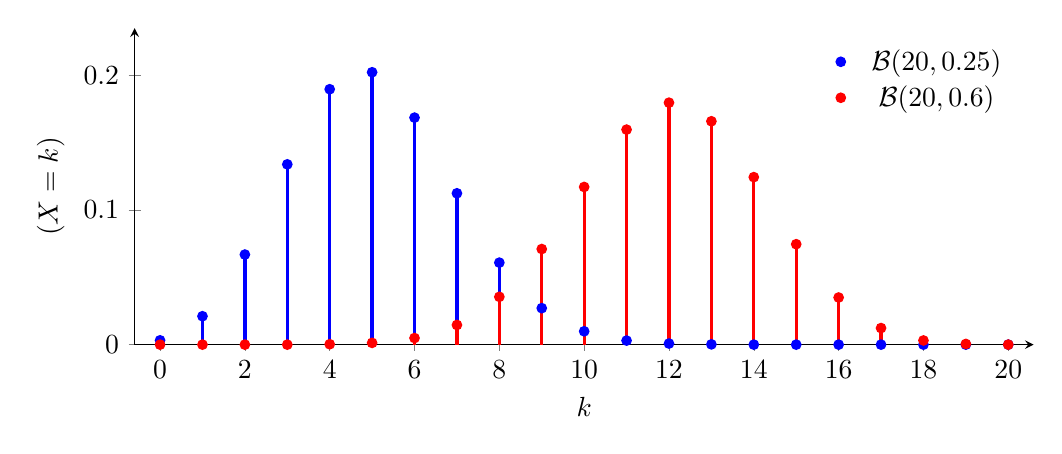
\begin{tikzpicture}
    \begin{axis}[width=13cm, height=5.6cm, axis lines=left,
      xlabel={$k$}, ylabel={$\prob(X = k)$},
      xmin=-0.6, xmax=20.6, ymin=0, ymax=0.235, xtick={0,2,4,6,8,10,12,14,16,18,20},
      legend style={at={(0.98,0.97)}, anchor=north east, draw=none}]
      \addplot[ycomb, very thick, mark=*, mark size=1.3pt, blue] coordinates {
        (0,0.0032) (1,0.0211) (2,0.0669) (3,0.1339) (4,0.1897) (5,0.2023)
        (6,0.1686) (7,0.1124) (8,0.0609) (9,0.0271) (10,0.0099) (11,0.0030)
        (12,0.0008) (13,0.0002) (14,0) (15,0) (16,0) (17,0) (18,0) (19,0) (20,0) };
      \addlegendentry{$\mathcal{B}(20, 0.25)$}
      \addplot[ycomb, very thick, mark=*, mark size=1.3pt, red] coordinates {
        (0,0) (1,0) (2,0) (3,0) (4,0.0003) (5,0.0013) (6,0.0049) (7,0.0146)
        (8,0.0355) (9,0.0710) (10,0.1171) (11,0.1597) (12,0.1797) (13,0.1659)
        (14,0.1244) (15,0.0746) (16,0.0350) (17,0.0123) (18,0.0031) (19,0.0005) (20,0) };
      \addlegendentry{$\mathcal{B}(20, 0.6)$}
    \end{axis}
  \end{tikzpicture}
\end{figure}

Both binomials above have $n = 20$. The mass concentrates around $np$ --- $5$ and
$12$ respectively --- and the spread is governed by $np(1-p)$, which is largest
at $p = \tfrac12$; the right-hand loi, being nearer the symmetric case,
is the wider of the two.

\begin{figure}[h!]
  \centering
  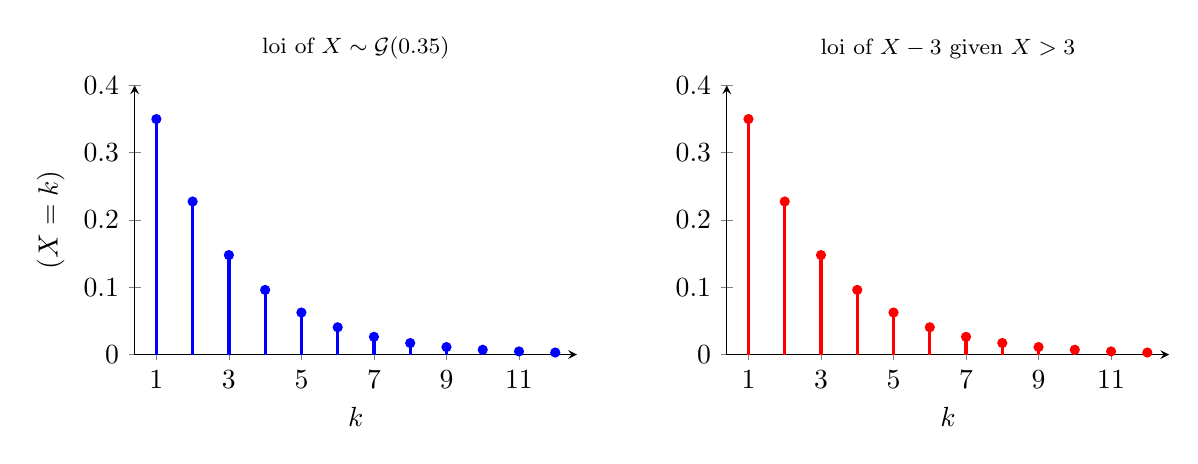
\begin{tikzpicture}
    \begin{axis}[name=left, width=7.2cm, height=5.0cm, axis lines=left,
      xlabel={$k$}, ylabel={$\prob(X = k)$},
      title={\footnotesize loi of $X \sim \mathcal{G}(0.35)$},
      xmin=0.4, xmax=12.6, ymin=0, ymax=0.40, xtick={1,3,5,7,9,11}]
      \addplot[ycomb, very thick, mark=*, mark size=1.2pt, blue] coordinates {
        (1,0.3500) (2,0.2275) (3,0.1479) (4,0.0961) (5,0.0625) (6,0.0406)
        (7,0.0264) (8,0.0172) (9,0.0112) (10,0.0072) (11,0.0047) (12,0.0031) };
    \end{axis}
    \begin{axis}[at={(left.right of origin)}, anchor=left of origin, xshift=1.9cm,
      width=7.2cm, height=5.0cm, axis lines=left, xlabel={$k$},
      title={\footnotesize loi of $X - 3$ given $X > 3$},
      xmin=0.4, xmax=12.6, ymin=0, ymax=0.40, xtick={1,3,5,7,9,11}]
      \addplot[ycomb, very thick, mark=*, mark size=1.2pt, red] coordinates {
        (1,0.3500) (2,0.2275) (3,0.1479) (4,0.0961) (5,0.0625) (6,0.0406)
        (7,0.0264) (8,0.0172) (9,0.0112) (10,0.0072) (11,0.0047) (12,0.0031) };
    \end{axis}
  \end{tikzpicture}
\end{figure}

The two panels are the same picture: this is the \textbf{absence de mémoire}
(\textit{memorylessness}) of the loi géométrique. Since
$\prob(X > k) = (1-p)^{k}$ on the support $\mathbb{N}^{*}$,
\[ \prob(X > n + k \mid X > n)
     = \frac{(1-p)^{n+k}}{(1-p)^{n}} = (1-p)^{k} = \prob(X > k). \]
Three failed trials leave the number of further trials distributed exactly as at
the start. The geometric is the only discrete loi with this property; the loi
exponentielle of chapter 4 is its continuous counterpart.

\subsection{Loi conditionnelle}

Soit $X$ une variable aléatoire à valeurs dans $E$.

\begin{definition}[Loi conditionnelle]
  Soit $A$ un événement tel que $\prob(A) > 0$. On appelle \textbf{loi
  conditionnelle} (\textit{conditional distribution}) de $X$ sachant $A$ la
  mesure de probabilité $\prob_{X \mid A}$ définie sur $E$ par :
  \[ \forall B \subr E, \qquad \prob_{X \mid A}(B) = \prob(X \in B \mid A). \]
\end{definition}

C'est la mesure image de la probabilité conditionnelle $\prob(\cdot \mid A)$ par
$X$. As before $\prob(A) > 0$ is what makes the definition legitimate; chapter 5
removes it, at the cost of defining the loi conditionnelle only up to a
négligeable set.

\begin{example}[Restricting a uniform die]
  Soit $X$ une variable aléatoire de loi uniforme sur $\{1,\dots,6\}$. La loi
  conditionnelle de $X$ sachant $X \le 3$ est une loi uniforme sur $\{1,2,3\}$.
  Each surviving value keeps the weight $\tfrac16$, and renormalising by
  $\prob(X \le 3) = \tfrac12$ turns it into $\tfrac13$. Conditioning a loi
  uniforme on a subset of its support gives the loi uniforme on that subset ---
  only because the weights were equal to begin with.
\end{example}

\subsection{Loi jointe, lois marginales}

Soit $X$ et $Y$ deux variables aléatoires à valeurs respectives dans $E$ et $F$.
Le couple $(X,Y)$ définit une variable aléatoire sur $E \times F$.

\begin{definition}[Loi jointe, lois marginales]
  La loi du couple $(X,Y)$, notée $\prob_{X,Y}$, est appelée la \textbf{loi
  jointe} (\textit{joint distribution}) de $X$ et $Y$. Les lois $\prob_{X}$ et
  $\prob_{Y}$ sont les \textbf{lois marginales} (\textit{marginal distributions})
  du couple.
\end{definition}

La loi jointe est une mesure de probabilité discrète, entièrement caractérisée
par ses valeurs sur les singletons :
\[ \forall x \in E,\ \forall y \in F, \qquad
   \prob_{X,Y}(\{x\} \times \{y\}) = \prob(X = x, Y = y), \]
et les lois marginales s'en déduisent, by summing out the other coordinate :
\[ \prob_{X}(x) = \sum_{y \in F} \prob(X = x, Y = y), \qquad
   \prob_{Y}(y) = \sum_{x \in E} \prob(X = x, Y = y). \]
The converse fails: the lois marginales do not determine the loi jointe, which
is what makes the next definition non-trivial.

\begin{definition}[Indépendance de deux variables aléatoires]
  Deux variables aléatoires $X$ et $Y$ sont dites \textbf{indépendantes} si pour
  tous $A \subr E$ et $B \subr F$, les événements $\{X \in A\}$ et
  $\{Y \in B\}$ sont indépendants, soit :
  \[ \prob(X \in A, Y \in B) = \prob(X \in A)\,\prob(Y \in B). \]
\end{definition}

\begin{prop}
  Deux variables aléatoires $X$ et $Y$ sont indépendantes si et seulement si
  \[ \forall x \in E,\ \forall y \in F, \qquad
     \prob(X = x, Y = y) = \prob(X = x)\prob(Y = y). \]
\end{prop}

Though indépendance quantifies over all pairs of subsets, la loi du couple étant
une loi discrète, il suffit de vérifier cette propriété sur les singletons;
summing recovers the general case. De façon équivalente,
les variables aléatoires $X$ et $Y$ sont indépendantes si et seulement si pour
tout $x \in E$ tel que $\prob(X=x) > 0$, la loi conditionnelle de $Y$ sachant
$X = x$ est la loi de $Y$.

\begin{prop}
  Si les variables aléatoires $X$ et $Y$ sont indépendantes, alors les
  variables aléatoires $\phi(X)$ et $\psi(Y)$ sont indépendantes, quelles que
  soient les fonctions $\phi$ et $\psi$.
\end{prop}

No hypothesis at all is needed on $\phi$ and $\psi$; in chapter 4 they must be
mesurables, which is the only change.

\begin{example}[Thinning a Poisson count by a fair coin]
  Une tortue donne naissance à $N$ bébés. On suppose que $N$ suit une loi de
  Poisson $\mathcal{P}(\lambda)$. Chaque bébé a une chance sur deux
  ($\tfrac{1}{2}$) d'être une femelle, independently of the others. On note $F$
  le nombre de bébés femelles.\\

  Conditionally on $N = n$, the variable $F$ counts the successes among $n$
  independent fair trials: sa loi conditionnelle est une loi binomiale
  $\mathcal{B}(n, \tfrac12)$. La loi jointe du couple est :
  \[ \forall 0 \le k \le n, \qquad
     \prob(N = n, F = k) = \prob(N=n)\prob(F = k \mid N = n)
       = e^{-\lambda} \frac{\lambda^{n}}{n!} \binom{n}{k} \frac{1}{2^{n}}. \]
  Summing over $n \ge k$, and substituting $m = n-k$,
  \[ \prob(F = k) = e^{-\lambda} \left(\frac{\lambda}{2}\right)^{k}
       \frac{1}{k!} \sum_{m \ge 0} \left(\frac{\lambda}{2}\right)^{m}
       \frac{1}{m!}
     = e^{-\lambda/2} \left(\frac{\lambda}{2}\right)^{k} \frac{1}{k!}, \]
  so $F$ follows the loi de Poisson $\mathcal{P}(\lambda/2)$. Thinning a
  Poisson count keeps it Poisson and halves the parameter.\\

  Les variables ne sont \emph{pas} indépendantes car la loi de $F$ sachant
  $N = 0$ est un Dirac en $0$, qui est différente de la loi de $F$. Having the
  same family of lois is no substitute for checking the product identity.
\end{example}

\subsection{Espérance}

Soit $X$ une variable aléatoire à valeurs réelles.

\begin{definition}[Espérance]
  L'\textbf{espérance} (\textit{expectation}) de la variable aléatoire $X$ est la
  valeur, éventuellement infinie,
  \[ \expec(X) = \sum_{\omega \in \Omega} X(\omega)\prob(\omega), \]
  pourvu que $X$ soit positive ou que $\expec(|X|) < \infty$.
\end{definition}

The proviso is the whole hypothesis. A sum over a countable index set is
order-independent only when its terms are positive or the sum is absolutely
convergent; without one of the two, $\expec(X)$ is not even well-defined. Every
manipulation below rests on it.

\begin{prop}
  L'espérance de la variable aléatoire $X$ dépend uniquement de sa loi :
  \[ \expec(X) = \sum_{x \in E} x \, \prob(X = x), \]
  pourvu que $X$ soit positive ou que $\expec(|X|) < \infty$.
\end{prop}

Une variable aléatoire d'espérance nulle est dite \textbf{centrée}
(\textit{centred}).

\begin{example}[The espérance of an indicator is a probability]
  Soit $A \subr \Omega$ un événement. Alors la variable aléatoire
  $X = \indic_{A}$ suit une loi de Bernoulli $\mathcal{B}(\prob(A))$, de sorte
  que
  \[ \expec(\indic_{A}) = \prob(A). \]
  This one line is the bridge between counting and probability, and it is the
  engine of the linearity arguments below.
\end{example}

\begin{example}[Espérances des cinq lois]
  L'espérance d'une variable aléatoire $X \sim \mathcal{B}(p)$ est
  $\expec(X) = \prob(X=1) = p$.\\

  L'espérance d'une variable aléatoire $X \sim \mathcal{P}(\lambda)$ est
  \[ \expec(X) = \sum_{k \ge 0} k\, e^{-\lambda} \frac{\lambda^{k}}{k!}
       = \lambda e^{-\lambda} \sum_{k \ge 1} \frac{\lambda^{k-1}}{(k-1)!}
       = \lambda. \]
  L'espérance d'une variable aléatoire $X \sim \mathcal{U}(1,\dots,n)$ est
  $\expec(X) = \frac{1+2+\dots+n}{n} = \frac{n+1}{2}$.\\

  For $X \sim \mathcal{B}(n,p)$, writing $X = \sum_{i=1}^{n} X_{i}$ with the
  $X_{i}$ independent $\mathcal{B}(p)$ and using linearity below,
  $\expec(X) = np$. For $X \sim \mathcal{G}(p)$,
  \[ \expec(X) = \sum_{k \ge 1} k(1-p)^{k-1} p
       = p \cdot \frac{1}{p^{2}} = \frac{1}{p}, \]
  using $\sum_{k \ge 1} k q^{k-1} = (1-q)^{-2}$ for $|q| < 1$.
\end{example}

\begin{theorem}[Transfert (\textit{transfer theorem})]
  Soit $X$ une variable aléatoire à valeurs dans $E$. Pour toute fonction
  $\phi : E \to \reals$,
  \[ \expec(\phi(X)) = \sum_{x \in E} \phi(x) \prob(X = x), \]
  pourvu que $\phi$ soit positive ou que $\expec(|\phi(X)|) < \infty$.
\end{theorem}

To compute the espérance of $\phi(X)$ one never needs $\Omega$: the loi of $X$
suffices, which is why a variable can be described by its loi alone. The
hypothesis is again positivity \emph{or} integrability, and it bears on
$\phi(X)$, not on $X$: $X$ may be integrable while $X^{2}$ is not.

\begin{corollary}[Linéarité]
  Soit $X$, $Y$ deux variables aléatoires réelles d'espérances finies. Alors,
  \[ \forall \alpha \in \reals, \quad \expec(\alpha X) = \alpha \expec(X),
     \qquad \text{and} \qquad
     \expec(X+Y) = \expec(X) + \expec(Y). \]
\end{corollary}

\begin{remark}
  Linearity requires \emph{finite} espérances and nothing else: $X$ and $Y$ need
  not be independent, so $\expec(X+Y) = \expec(X) + \expec(Y)$ holds for
  arbitrarily dependent variables. On raisonne en appliquant le théorème de
  transfert au couple $(X,Y)$, the absolute convergence coming from the
  finiteness hypothesis. Contrast the product rule below, which does need
  indépendance, and the variance of a sum, which does not split without it.
\end{remark}

\begin{prop}[Espérance d'une série]
  Pour toute suite de variables aléatoires réelles $(X_{n})_{n \ge 1}$,
  \[ \expec\left( \sum_{n \ge 1} X_{n} \right) = \sum_{n \ge 1} \expec(X_{n}) \]
  dès que les variables aléatoires $X_{n}$ sont positives pour tout $n \ge 1$ ou
  que $\sum_{n \ge 1} \expec(|X_{n}|) < \infty$.
\end{prop}

This is linearity extended to a countable sum, and the discrete form of the
convergence monotone and convergence dominée theorems of chapter 3. The second
hypothesis bounds the \emph{sum} of the $\expec(|X_{n}|)$, not each term
separately.

\begin{prop}
  Pour toutes variables aléatoires réelles $X$, $Y$ indépendantes d'espérances
  finies,
  \[ \expec(XY) = \expec(X)\expec(Y). \]
\end{prop}

Indépendance is essential; finiteness of $\expec(X)$ and $\expec(Y)$ then gives
$\expec(|XY|) = \expec(|X|)\expec(|Y|) < \infty$, so $XY$ is automatically
integrable. The converse is false: $\expec(XY) = \expec(X)\expec(Y)$ says only
that $X$ and $Y$ are décorrélées, which is weaker than indépendance.

\begin{example}[Fixed points of a random ordering, by indicators and linearity]
  One object here is borrowed from chapter 4 and one is not: the variables to be
  sorted are continuous, and so outside this chapter, but the permutation that
  sorts them takes finitely many values, so it is a discrete variable aléatoire
  and the computation below lives entirely in the present setting.\\

  Let $X_{1}, \dots, X_{n}$ be \textbf{indépendantes et identiquement
  distribuées} (\textit{independent and identically distributed}) real variables
  aléatoires, abbreviated i.i.d.\ from here on, whose common
  loi has a densité --- an object chapter 4 builds, quoted here only for
  the one fact that $\prob(X_{i} = X_{j}) = 0$ for $i \ne j$;
  by the borne de l'union, $\prob(\exists i \ne j,\ X_{i} = X_{j}) = 0$. There
  is therefore presque sûrement a unique permutation $\sigma$ of
  $\{1,\dots,n\}$ that sorts them,
  $X_{\sigma(1)} < \dots < X_{\sigma(n)}$, and $\sigma$ is a variable aléatoire
  with values in the set of permutations.\\

  Because the $X_{i}$ are i.i.d., for every fixed permutation $s$,
  \[ \prob(\sigma = s) = \prob(X_{s(1)} < \dots < X_{s(n)})
                       = \prob(X_{1} < \dots < X_{n}), \]
  a quantity that does not depend on $s$, so $\sigma$ is uniform on the $n!$
  permutations. In particular $\prob(\sigma(i) = j) = \tfrac1n$ for all $i,j$.\\

  How many fixed points does $\sigma$ have on average? Write the count as a sum
  of indicators and use linearity:
  \[ \expec\left( \sum_{i=1}^{n} \indic_{\{\sigma(i) = i\}} \right)
       = \sum_{i=1}^{n} \expec(\indic_{\{\sigma(i)=i\}})
       = \sum_{i=1}^{n} \prob(\sigma(i) = i)
       = n \cdot \frac{1}{n} = 1. \]
  The answer is $1$ for every $n$, and the événements $\{\sigma(i)=i\}$ are
  heavily dependent --- knowing $n-1$ of them determines the last --- which
  linearity does not care about. The method is the one to keep for any counting
  espérance: decompose into indicators, take espérances termwise, read each term
  as a probability.
\end{example}

\subsection{Variance, covariance}

Soit $X$ une variable aléatoire réelle d'espérance finie.

\begin{definition}[Variance]
  La \textbf{variance} de la variable aléatoire $X$ est la valeur, éventuellement
  infinie :
  \[ \Var(X) = \expec\big( (X - \expec(X))^{2} \big). \]
\end{definition}

Par linéarité de l'espérance, on obtient l'expression équivalente :
\[ \Var(X) = \expec(X^{2}) - \expec(X)^{2}, \]
which is the one to compute with; it comes from expanding the square.

\begin{prop}
  On a $\Var(X) \ge 0$ avec $\Var(X) = 0$ si et seulement si $X = \expec(X)$ p.s.
\end{prop}

The abbreviation \textit{p.s.} means \textbf{presque sûrement} (\textit{almost
surely}), c'est-à-dire avec probabilité $1$; it is kept in its French form. Here it says
$X(\omega) = \expec(X)$ for every $\omega$ with $\prob(\omega) > 0$: the
values of $X$ on the null part of $\Omega$ are unconstrained, which is why the
conclusion is not $X = \expec(X)$ everywhere.\\

Par linéarité de l'espérance, on a :
\[ \forall \alpha \in \reals, \qquad \Var(\alpha X) = \alpha^{2} \Var(X). \]
The variance scales quadratically: the square is the entire content of the
rule, and the reason the écart type $\sqrt{\Var(X)}$, not the variance, is the
quantity with the same units as $X$. In particular $\Var(-X) = \Var(X)$, the case $\alpha = -1$. Separately,
$\Var(X + c) = \Var(X)$ for a constant $c$, which does not follow from the
scaling rule but straight from the definition: adding $c$ moves $X$ and
$\expec(X)$ by the same amount, so $X + c - \expec(X+c) = X - \expec(X)$.\\

On considère maintenant $X$ et $Y$ deux variables aléatoires de variances finies.

\begin{definition}[Covariance]
  La \textbf{covariance} entre les variables aléatoires $X$ et $Y$ est la
  valeur :
  \[ \Cov(X,Y) = \expec\big( (X - \expec(X))(Y - \expec(Y)) \big). \]
\end{definition}

Finiteness of the two variances is what makes this well-defined: on en déduit
que $\expec(X^{2}) < \infty$ et $\expec(Y^{2}) < \infty$. En utilisant le fait
que $|XY| \le \tfrac{1}{2}(X^{2} + Y^{2})$, on obtient que $XY$ est d'espérance
finie. Par linéarité de l'espérance --- after expanding the product --- on
obtient alors :
\[ \Cov(X,Y) = \expec(XY) - \expec(X)\expec(Y). \]
On note que $\Cov(X,Y) = 0$ dès que $X$ et $Y$ sont indépendantes. La
réciproque est fausse.\\

La covariance vérifie les propriétés suivantes :
\begin{itemize}
  \item $\Cov(X,X) = \Var(X)$;
  \item $\Cov(X,Y) = \Cov(Y,X)$;
  \item $\Cov(\alpha X, Y) = \alpha \Cov(X,Y)$ pour tout $\alpha \in \reals$;
  \item $\Cov(X, Y+Z) = \Cov(X,Y) + \Cov(X,Z)$ pour toutes variables $X,Y,Z$ de
    variances finies.
\end{itemize}
En particulier, la covariance est une forme bilinéaire symétrique.

\begin{remark}
  La covariance n'est \emph{pas} \textbf{définie positive} (\textit{positive
  definite}) car $\Var(X) = 0$ implique uniquement que $X$ est p.s.\ constante,
  not zero. La covariance n'est définie positive que si l'on se restreint aux
  variables aléatoires centrées --- identifying two that are p.s.\ equal. Elle
  définit alors un produit scalaire.
  That structure is the right way to see the next two results: the variance of a
  sum is an expansion of $\|X+Y\|^{2}$, and Cauchy--Schwartz is Cauchy--Schwartz.
\end{remark}

\begin{prop}
  On a pour toutes variables aléatoires $X$ et $Y$ de variances finies :
  \[ \Var(X+Y) = \Var(X) + 2\Cov(X,Y) + \Var(Y). \]
\end{prop}

\begin{corollary}
  Si les variables aléatoires $X$ et $Y$ sont indépendantes et de variances
  finies, alors $\Cov(X,Y) = 0$ et
  \[ \Var(X+Y) = \Var(X) + \Var(Y). \]
\end{corollary}

The cross term is the only place indépendance enters. Espérances add for any
pair of integrable variables; variances add only when the covariance vanishes,
and vanishing covariance is weaker than indépendance, so the corollary is
genuinely weaker than the proposition. With the scaling rule, for independent
$X, Y$ and reals $a, b$,
\[ \Var(aX + bY) = a^{2}\Var(X) + b^{2}\Var(Y), \]
the squares again.

\begin{prop}[Inégalité de Cauchy-Schwartz (\textit{Cauchy--Schwartz inequality})]
  On a pour toutes variables aléatoires $X$ et $Y$ de variances finies :
  \[ |\Cov(X,Y)| \le \sqrt{\Var(X)\Var(Y)}. \]
\end{prop}

The name is spelled \emph{Cauchy--Schwartz} throughout. On peut supposer les
variables aléatoires $X$ et $Y$ centrées, quitte à considérer les variables
$X - \expec(X)$ et $Y - \expec(Y)$, which changes neither side. Le résultat est
alors une conséquence du fait que la covariance définit un produit scalaire: the
inequality is Cauchy--Schwartz for the inner product of the remark above.

\begin{definition}[Coefficient de corrélation]
  Le \textbf{coefficient de corrélation} (\textit{correlation coefficient}) entre
  deux variables aléatoires $X$ et $Y$ de variances finies et non nulles est la
  valeur :
  \[ \rho(X,Y) = \frac{\Cov(X,Y)}{\sqrt{\Var(X)\Var(Y)}}. \]
\end{definition}

The variances must be non-zero for the quotient to exist --- a p.s.\ constant
variable has no correlation with anything. Au vu de l'inégalité de
Cauchy-Schwartz, on a $\rho(X,Y) \in [-1,1]$, avec $|\rho(X,Y)| = 1$ si et
seulement si $X$ et $Y$ sont linéairement dépendantes, à savoir
$\rho(X,Y) = 1$ si et seulement si $Y = aX+b$ avec $a > 0$, et
$\rho(X,Y) = -1$ si et seulement si $Y = aX+b$ avec $a < 0$. Lorsque
$\rho(X,Y) = 0$, on dit que les variables sont \textbf{décorrélées}
(\textit{uncorrelated}). The coefficient is
the cosine of the ``angle'' between the two variables centrées.

\begin{figure}[h!]
  \centering
  \begin{tikzpicture}
    \begin{axis}[name=p1, scale only axis, width=4.6cm, height=4.6cm,
      axis lines=middle,
      title={\footnotesize $\rho = -1$}, xtick=\empty, ytick=\empty,
      xmin=-1.4, xmax=1.4, ymin=-1.4, ymax=1.4]
      \addplot[only marks, mark=*, mark size=1.4pt, blue] coordinates {
        (-1.2,1.2) (-0.9,0.9) (-0.6,0.6) (-0.3,0.3) (0,0)
        (0.3,-0.3) (0.6,-0.6) (0.9,-0.9) (1.2,-1.2) };
    \end{axis}
    \begin{axis}[at={(p1.right of origin)}, anchor=left of origin, xshift=1.5cm,
      name=p2, scale only axis, width=4.6cm, height=4.6cm, axis lines=middle,
      title={\footnotesize $\rho = 0$, yet dependent}, xtick=\empty, ytick=\empty,
      xmin=-1.4, xmax=1.4, ymin=-1.4, ymax=1.4]
      \addplot[only marks, mark=*, mark size=1.4pt, red] coordinates {
        (1.0,0) (0.87,0.5) (0.5,0.87) (0,1.0) (-0.5,0.87) (-0.87,0.5) (-1.0,0)
        (-0.87,-0.5) (-0.5,-0.87) (0,-1.0) (0.5,-0.87) (0.87,-0.5) };
    \end{axis}
    \begin{axis}[at={(p2.right of origin)}, anchor=left of origin, xshift=1.5cm,
      scale only axis, width=4.6cm, height=4.6cm, axis lines=middle,
      title={\footnotesize $\rho = +1$}, xtick=\empty, ytick=\empty,
      xmin=-1.4, xmax=1.4, ymin=-1.4, ymax=1.4]
      \addplot[only marks, mark=*, mark size=1.4pt, blue] coordinates {
        (-1.2,-1.2) (-0.9,-0.9) (-0.6,-0.6) (-0.3,-0.3) (0,0)
        (0.3,0.3) (0.6,0.6) (0.9,0.9) (1.2,1.2) };
    \end{axis}
  \end{tikzpicture}
\end{figure}

The outer panels are the extreme cases: all the mass on a line, $\rho = \pm 1$ by
the slope's sign. The middle panel is the one to remember --- the mass is uniform
on a circle, so by symmetry $\expec(X) = \expec(Y) = \expec(XY) = 0$ and the
coordinates are décorrélées, yet $X$ determines $Y$ up to a sign. Correlation
measures only the \emph{linear} part of a dependence, so $\rho = 0$ is strictly
weaker than indépendance.

\begin{example}[Uncorrelated but not independent]
  Soit $X$ une variable aléatoire de loi uniforme sur $\{0,1\}$ et $Z$ une
  variable aléatoire de loi uniforme sur $\{-1,+1\}$ indépendante de $X$. On note
  $Y = XZ$. Since $\expec(Z) = 0$ and $Z$ is independent of $X$ and
  of $X^{2}$,
  \[ \expec(Y) = \expec(XZ) = \expec(X)\expec(Z) = 0, \qquad
     \expec(XY) = \expec(X^{2}Z) = \expec(X^{2})\expec(Z) = 0, \]
  so $\Cov(X,Y) = \expec(XY) - \expec(X)\expec(Y) = 0$ and the variables are
  décorrélées. Par contre, $\prob(X=0, Y=1) = 0$ tandis que
  $\prob(X=0) = \tfrac12$ et $\prob(Y=1) = \tfrac14$, donc les variables ne sont
  pas indépendantes: the product identity fails on a single pair of singletons.
  One pair suffices to break indépendance.
\end{example}

\begin{example}[Variances des cinq lois]
  For $X \sim \mathcal{B}(p)$, $X^{2} = X$ so
  $\Var(X) = p - p^{2} = p(1-p)$.\\

  For $X \sim \mathcal{B}(n,p)$, write $X$ as a sum of $n$ independent Bernoulli
  variables; the covariances vanish and the variances add, giving
  $\Var(X) = np(1-p)$. This is the corollary above doing real work: the
  summands are not identically zero, but their pairwise covariances are.\\

  For $X \sim \mathcal{P}(\lambda)$, $\expec(X(X-1)) = \lambda^{2}$, so
  $\expec(X^{2}) = \lambda^{2} + \lambda$ and $\Var(X) = \lambda$: the loi de
  Poisson has equal mean and variance. For $X \sim \mathcal{G}(p)$,
  $\Var(X) = \frac{1-p}{p^{2}}$, and for $X \sim \mathcal{U}(1,\dots,n)$,
  $\Var(X) = \frac{n^{2}-1}{12}$.
\end{example}

\subsection{Fonction génératrice}

La fonction génératrice d'une variable aléatoire à valeurs entières positives
permet de caractériser la loi et d'en calculer les moments.

\begin{definition}[Fonction génératrice]
  La \textbf{fonction génératrice} (\textit{generating function}) d'une variable
  aléatoire $X$ à valeurs dans $\mathbb{N}$ est la fonction $G_{X}$ définie
  par :
  \[ \forall t \in [-1,1], \qquad
     G_{X}(t) = \expec(t^{X}) = \sum_{k \ge 0} \prob(X = k)\, t^{k}. \]
\end{definition}

The hypothesis that $X$ takes values in $\mathbb{N}$ is what the construction
needs: $t^{X}$ must be a power series in $t$. Il s'agit d'une série entière de
rayon de convergence supérieur ou égal à $1$ --- the coefficients sum to $1$ ---
et $G_{X}$ est donc une fonction continue sur $[-1,1]$ et $C^{\infty}$ sur
$]-1,1[$. The endpoints are the delicate ones, and the one-sided derivative at
$1$ below is where the moments live.

\begin{prop}
  On a $\prob(X = 0) = G_{X}(0)$ et pour tout $k \ge 1$,
  \[ \prob(X = k) = \frac{1}{k!} \frac{d^{k} G_{X}}{dt^{k}}(0). \]
\end{prop}

Ce résultat montre que la fonction génératrice caractérise la loi: two
$\mathbb{N}$-valued variables with the same fonction génératrice have the same
loi. That is the first of its two uses.\\

The second is moments. La fonction génératrice a toujours une dérivée à gauche
en $1$, éventuellement infinie, et on a :
\[ \expec(X) = G_{X}'(1^{-}). \]
More generally the $k$-th \textbf{factorial moment} is read off the $k$-th
left derivative, when that derivative is finite:
\[ \expec\big( X(X-1)\cdots(X-k+1) \big)
     = \frac{d^{k} G_{X}}{dt^{k}}(1^{-}). \]
The derivative is a \emph{left} derivative at $1$, since $G_{X}$ is only defined
on $[-1,1]$, and it may be infinite --- exactly when $X$ has no moment of that
order. From the factorial moments the ordinary ones follow:
$\expec(X^{2}) = G_{X}''(1^{-}) + G_{X}'(1^{-})$, and then
$\Var(X) = G_{X}''(1^{-}) + G_{X}'(1^{-}) - G_{X}'(1^{-})^{2}$.

\begin{prop}
  Soit $X$, $Y$ deux variables aléatoires indépendantes à valeurs dans
  $\mathbb{N}$. Alors,
  \[ G_{X+Y} = G_{X} G_{Y}. \]
\end{prop}

The proof is one line --- $\expec(t^{X+Y}) = \expec(t^{X})\expec(t^{Y})$ by
indépendance --- and the consequence is that a convolution of lois becomes a
product of functions. Indépendance is indispensable; without it the espérance of
the product does not factor.

\begin{remark}
  These two properties are exactly what makes the fonction caractéristique
  $\varphi_{X}$ of chapter 6 worth building: $\varphi_{X}(t) = \expec(e^{itX})$
  characterises the loi of \emph{any} real variable aléatoire, its
  derivatives at $0$ give the moments, and $\varphi_{X+Y} = \varphi_{X}\varphi_{Y}$ for
  independent summands. The fonction génératrice is the same idea restricted to
  $\mathbb{N}$-valued variables, with $t$ for $e^{it}$: cheaper, real-valued, and
  enough whenever the variable counts something.
\end{remark}

\begin{example}[Fonctions génératrices des cinq lois]
  La fonction génératrice d'une variable aléatoire $X \sim \mathcal{B}(p)$ est
  $G_{X}(t) = 1 - p + pt$. For
  $X \sim \mathcal{B}(n,p)$, the binomial is a sum of $n$ independent Bernoulli
  variables, so the product rule gives $G_{X}(t) = (1-p+pt)^{n}$ at once.\\

  La fonction génératrice d'une variable aléatoire $X \sim \mathcal{P}(\lambda)$
  est
  \[ G_{X}(t) = \sum_{k \ge 0} e^{-\lambda} \frac{\lambda^{k}}{k!} t^{k}
       = e^{-\lambda} e^{\lambda t} = e^{\lambda(t-1)}. \]
  For $X \sim \mathcal{G}(p)$, summing the geometric series,
  $G_{X}(t) = \frac{pt}{1 - (1-p)t}$, which is finite for every
  $t \in [-1,1]$ when $p \in\, ]0,1]$. For $X \sim \mathcal{U}(1,\dots,n)$,
  $G_{X}(t) = \frac{t}{n}\frac{1-t^{n}}{1-t}$ for $t \ne 1$, and $G_{X}(1) = 1$.
\end{example}

\begin{example}[The sum of two independent Poisson counts]
  Soit $X$, $Y$ des variables aléatoires indépendantes suivant des lois de
  Poisson $\mathcal{P}(\alpha)$ et $\mathcal{P}(\beta)$. Then
  \[ G_{X+Y}(t) = G_{X}(t)G_{Y}(t)
       = e^{\alpha(t-1)} e^{\beta(t-1)} = e^{(\alpha+\beta)(t-1)}, \]
  which is the fonction génératrice of $\mathcal{P}(\alpha+\beta)$. Since the
  fonction génératrice characterises the loi, $X + Y \sim
  \mathcal{P}(\alpha+\beta)$. Computing the same convolution directly means
  summing $\sum_{j} \prob(X=j)\prob(Y=k-j)$ and recognising a binomial
  expansion; the fonction génératrice makes it a product of exponentials.
\end{example}

\begin{center}
  \begin{tabular}{lcccc}
    \toprule
    Loi & Support & $\expec(X)$ & $\Var(X)$ & $G_{X}(t)$ \\
    \midrule
    $\mathcal{B}(p)$ & $\{0,1\}$ & $p$ & $p(1-p)$ & $1-p+pt$ \\[2pt]
    $\mathcal{B}(n,p)$ & $\{0,\dots,n\}$ & $np$ & $np(1-p)$ & $(1-p+pt)^{n}$ \\[2pt]
    $\mathcal{P}(\lambda)$ & $\mathbb{N}$ & $\lambda$ & $\lambda$ & $e^{\lambda(t-1)}$ \\[2pt]
    $\mathcal{G}(p)$ & $\mathbb{N}^{*}$ & $\dfrac{1}{p}$ & $\dfrac{1-p}{p^{2}}$ & $\dfrac{pt}{1-(1-p)t}$ \\[4pt]
    $\mathcal{U}(1,\dots,n)$ & $\{1,\dots,n\}$ & $\dfrac{n+1}{2}$ & $\dfrac{n^{2}-1}{12}$ & $\dfrac{t}{n}\dfrac{1-t^{n}}{1-t}$ \\
    \bottomrule
  \end{tabular}
\end{center}

\begin{remark}
  The loi géométrique is the one to watch. This course puts its support on
  $\mathbb{N}^{*}$, counting the trials \emph{up to and including} the first
  success, so $\expec(X) = 1/p$; many computations instead use $\tau = X - 1$, the
  failures \emph{before} the first success, supported on $\mathbb{N}$, with
  $\expec(\tau) = (1-p)/p$. Check which of the two is meant before quoting a mean.
\end{remark}

\begin{example}[Surviving hatchlings, by composing fonctions génératrices]
  Une tortue donne naissance à $N$ bébés. On suppose que
  $N \sim \mathcal{P}(\lambda)$. Chaque bébé a une probabilité de survivre
  $p \in\, ]0,1[$, indépendamment des autres bébés. On note $X$ le nombre de
  bébés tortues qui survivent.\\

  The fonction génératrice of $N$ is $G_{N}(t) = e^{\lambda(t-1)}$. Conditioning
  on $N = n$ and using the product rule for the $n$ independent Bernoulli
  survival indicators, whose common fonction génératrice is $G(t) = 1 - p + pt$,
  \[ G_{X}(t) = \sum_{n \ge 0} \prob(N=n) \expec(t^{X} \mid N = n)
       = \sum_{n \ge 0} \prob(N=n) G(t)^{n}
       = G_{N}(G(t)). \]
  Hence $G_{X}(t) = e^{\lambda(1-p+pt-1)} = e^{\lambda p (t-1)}$, the fonction
  génératrice of $\mathcal{P}(\lambda p)$, so $X \sim \mathcal{P}(\lambda p)$. The
  earlier computation was the case $p = \tfrac12$ done by summing the loi
  jointe; the composition $G_{N} \circ G$ --- the fonction génératrice of a random
  sum of i.i.d.\ variables --- does it for any $p$, and is what a branching
  process is built on.
\end{example}

\subsection{Espérance conditionnelle}

Soit $X$ une variable aléatoire à valeurs réelles.

\begin{definition}[Espérance conditionnelle]
  Pour tout événement $A$ tel que $\prob(A) > 0$, on appelle \textbf{espérance
  conditionnelle} (\textit{conditional expectation}) de la variable aléatoire
  $X$ sachant $A$ la valeur :
  \[ \expec(X \mid A) = \sum_{\omega \in \Omega} X(\omega) \prob(\omega \mid A), \]
  pourvu que $X$ soit positive ou que $\expec(|X| \mid A) < \infty$.
\end{definition}

C'est l'espérance pour la probabilité conditionnelle $\prob(\cdot \mid A)$.
Everything proved about espérances therefore applies unchanged --- linearity,
the théorème de transfert, and the integrability proviso, which here is a
condition under the \emph{conditional} mesure.

\begin{prop}
  L'espérance conditionnelle de la variable aléatoire $X$ sachant $A$ s'obtient
  directement à partir de la loi conditionnelle :
  \[ \expec(X \mid A) = \sum_{x \in E} x\, \prob(X = x \mid A), \]
  pourvu que $X$ soit positive ou que $\expec(|X| \mid A) < \infty$.
\end{prop}

\begin{prop}
  L'espérance conditionnelle de la variable aléatoire $X$ sachant $A$ vérifie :
  \[ \expec(X \mid A) = \frac{\expec(X \indic_{A})}{\prob(A)}. \]
\end{prop}

This identity is the practical one: it replaces a conditional mesure by an
ordinary espérance of a truncated variable. It is also the form that survives
into chapter 5, where an integral identity of this shape \emph{defines} the
loi conditionnelle and the espérance conditionnelle is then read off it as
an integral against that loi.

\begin{prop}
  Soit $(A_{i})_{i \in I}$ une famille d'événements formant une partition de
  $\Omega$, avec $\prob(A_{i}) > 0$ pour tout $i \in I$. Alors,
  \[ \expec(X) = \sum_{i \in I} \prob(A_{i}) \expec(X \mid A_{i}) \]
  dès que $X$ est positive ou $\expec(|X|) < \infty$.
\end{prop}

On en déduit l'équivalent de la formule des probabilités totales pour
l'espérance --- proved from the previous proposition together with
$\sum_{i \in I} \indic_{A_{i}} = 1$ and the espérance of a series. The
hypotheses accumulate rather than simplify: a partition, each part of positive
probability, and $X$ positive or integrable.

\begin{example}[Averaging a die over an even outcome]
  Soit $X$ une variable aléatoire de loi uniforme sur $\{1,\dots,6\}$.
  L'espérance conditionnelle est donnée par
  $\expec(X \mid X \text{ even}) = \sum_{k=1}^{6} k\,\prob(X=k \mid X \text{
  even}) = \tfrac{2+4+6}{3} = 4$, against $\expec(X) = 3.5$ unconditionally.
  Conditioning restricts the support and renormalises the weights; both effects
  move the mean.
\end{example}

\begin{example}[When to stop rolling: a threshold from espérances conditionnelles]
  Les règles du jeu sont les suivantes : on part d'un score nul ($0$). À chaque
  coup, on lance deux dés. Si le total vaut $7$, le score retourne à $0$ et la
  partie est terminée ; sinon, le score augmente du total obtenu et on a le droit
  de rejouer. Si l'on ne rejoue pas, le score est acquis et la partie est
  terminée. On note $X$ le total obtenu sur un lancer, et $(X_{n})_{n \ge 0}$ une
  suite de variables aléatoires i.i.d.\ de même loi que $X$.\\

  The loi of $X$ is the familiar triangle on $\{2,\dots,12\}$, with
  $\prob(X = k) = \tfrac{1}{36}\min(k-1, 13-k)$, and $\expec(X) = 7$ by symmetry
  about $7$. Soit $\tau = \inf\{n \ge 0 : X_{n} = 7\}$: it is the number of
  throws before the first $7$. Since $\prob(X = 7) = \tfrac16$, the variable
  $\tau + 1$ is geometric $\mathcal{G}(\tfrac16)$, so
  $\expec(\tau) = \tfrac{1}{1/6} - 1 = 5$.\\

  A player who knew the next throw in advance would stop just before the $7$,
  scoring $S = \sum_{n=0}^{\tau - 1} X_{n}$. Conditioning on $\tau$ and using the
  formule des probabilités totales for espérances,
  \[ \expec(S) = \sum_{t \ge 1} \prob(\tau = t)\, t\, \expec(X \mid X \ne 7)
       = \expec(\tau)\, \expec(X \mid X \ne 7) = 5 \times 7 = 35, \]
  where $\expec(X \mid X \ne 7) = \expec(X) = 7$ because the triangle is
  symmetric about $7$, so removing the value $7$ does not move the mean.\\

  For an ordinary player at score $s$, throwing again gives
  \[ \expec(S_{n+1} \mid S_{n} = s)
       = \prob(X \ne 7)\,\big( s + \expec(X \mid X \ne 7) \big)
       = \tfrac56 (s + 7), \]
  since with probability $\tfrac16$ the score is wiped out. Throwing is worth it
  exactly when $\tfrac56(s+7) > s$, that is when $s < 35$. La stratégie optimale
  consiste à jouer tant que l'on n'a pas atteint $35$, et à s'arrêter après avoir
  franchi ce seuil. The threshold is the clairvoyant's score again, and for the
  same reason: both are $\expec(X)(1-p)/p = \expec(X)\expec(\tau)$ with
  $p = \prob(X = 7)$.
\end{example}

\subsection{Vecteurs aléatoires}

Soit $E_{1}, \dots, E_{n}$ des ensembles au plus dénombrables.

\begin{definition}[Vecteur aléatoire]
  Un \textbf{vecteur aléatoire} (\textit{random vector}) est une variable
  aléatoire à valeurs dans l'espace produit $E = E_{1} \times \dots \times E_{n}$.
\end{definition}

Ses composantes $X_{1}, \dots, X_{n}$ sont des variables aléatoires à valeurs
respectives dans $E_{1}, \dots, E_{n}$. La loi du vecteur $X$ est appelée la loi
jointe des variables aléatoires $X_{1}, \dots, X_{n}$ ; les lois
$\prob_{X_{1}}, \dots, \prob_{X_{n}}$ en sont les lois marginales. Elles s'en
déduisent en sommant sur toutes les autres variables.

\begin{example}[Loi multinomiale]
  Soit $X$ une variable aléatoire de \textbf{loi multinomiale}
  (\textit{multinomial distribution}) de paramètres $(N, p_{1}, \dots, p_{n})$
  avec $p_{1} + \dots + p_{n} = 1$ :
  \[ \forall x \in \mathbb{N}^{n} \text{ with } x_{1} + \dots + x_{n} = N,
     \qquad \prob(X = x)
       = \frac{N!}{x_{1}! \cdots x_{n}!} p_{1}^{x_{1}} \cdots p_{n}^{x_{n}}. \]
  C'est un vecteur aléatoire. It counts how many of $N$ independent trials fall
  into each of $n$ categories. Les lois marginales sont des lois binomiales:
  looking at one category only turns the other $n-1$ into a single ``failure''
  category, so $X_{i} \sim \mathcal{B}(N, p_{i})$.
\end{example}

\begin{definition}[Fonction génératrice vectorielle (\textit{vector generating function})]
  La \textbf{fonction génératrice} d'un vecteur aléatoire $X$ à valeurs dans
  $\mathbb{N}^{n}$ est la fonction $G_{X}$ définie par :
  \[ \forall t \in [-1,1]^{n}, \qquad
     G_{X}(t) = \expec(t_{1}^{X_{1}} \cdots t_{n}^{X_{n}})
       = \sum_{k_{1}, \dots, k_{n} \ge 0}
         \prob(X_{1} = k_{1}, \dots, X_{n} = k_{n})\,
         t_{1}^{k_{1}} \cdots t_{n}^{k_{n}}. \]
\end{definition}

Comme dans le cas des variables aléatoires, la fonction génératrice caractérise
la loi, et permet d'obtenir les moments par dérivations successives ---
\emph{partial} ones, now including the mixed ones, which is what makes it a tool
for covariances rather than just for variances.

\begin{example}[Covariance inside a multinomial, from the fonction génératrice vectorielle]
  For the loi multinomiale with parameters $(N, p_{1}, \dots, p_{n})$, the
  multinomial theorem collapses the sum:
  \[ \forall t \in [-1,1]^{n}, \qquad
     G_{X}(t) = (p_{1}t_{1} + \dots + p_{n}t_{n})^{N}. \]
  Differentiating at $t = (1, \dots, 1)$, where $p_{1} + \dots + p_{n} = 1$
  makes the base equal to $1$,
  \[ \expec(X_{i}) = \frac{\partial G_{X}}{\partial t_{i}}(1) = N p_{i},
     \qquad
     \expec(X_{i}X_{j})
       = \frac{\partial^{2} G_{X}}{\partial t_{i} \partial t_{j}}(1)
       = N(N-1) p_{i}p_{j} \quad (i \ne j), \]
  the second being a mixed partial, so it returns $\expec(X_{i}X_{j})$ rather
  than a factorial moment. Hence
  \[ \Cov(X_{i}, X_{j}) = N(N-1)p_{i}p_{j} - N^{2}p_{i}p_{j} = -N p_{i}p_{j}. \]
  The same derivative taken twice in $t_{i}$ gives the factorial moment
  $\expec(X_{i}(X_{i}-1)) = N(N-1)p_{i}^{2}$, whence
  $\Var(X_{i}) = Np_{i}(1-p_{i})$, consistent with the binomial loi marginale,
  and
  \[ \rho(X_{i}, X_{j})
       = -\sqrt{\frac{p_{i}}{1-p_{i}} \cdot \frac{p_{j}}{1-p_{j}}}. \]
  The correlation is negative for every pair, as it must be: the $N$ trials are
  shared out, so a trial counted in category $i$ is one that category $j$ cannot
  have.
\end{example}

\subsection{Variables aléatoires indépendantes}

\begin{definition}[Indépendance d'une famille]
  Les variables aléatoires $X_{1}, \dots, X_{n}$ sont dites
  \textbf{indépendantes} si pour tous $A_{1} \subr E_{1}, \dots, A_{n} \subr E_{n}$,
  les événements $\{X_{1} \in A_{1}\}, \dots, \{X_{n} \in A_{n}\}$ sont
  indépendants.
\end{definition}

Pour vérifier l'indépendance, il suffit donc de s'assurer que :
\[ \prob(X_{1} \in A_{1}, \dots, X_{n} \in A_{n})
     = \prob(X_{1} \in A_{1}) \cdots \prob(X_{n} \in A_{n}) \]
pour tous $A_{1} \subr E_{1}, \dots, A_{n} \subr E_{n}$. Si l'indépendance d'une
famille d'événements exige de regarder tous les sous-ensembles finis de ces
événements, ceci est fait de façon implicite ici grâce au choix des ensembles
$A_{i}$ : le choix $A_{1} = E_{1}$ par exemple élimine le premier événement,
which it makes certain and so drops from the product. Running each $A_{i}$ over
subsets and over $E_{i}$ therefore covers all sub-families.

\begin{prop}
  Les variables aléatoires $X_{1}, \dots, X_{n}$ sont indépendantes si et
  seulement si :
  \[ \forall x_{1} \in E_{1}, \dots, \forall x_{n} \in E_{n}, \qquad
     \prob(X_{1} = x_{1}, \dots, X_{n} = x_{n})
       = \prob(X_{1} = x_{1}) \cdots \prob(X_{n} = x_{n}). \]
\end{prop}

\begin{prop}
  Si les variables aléatoires $X_{1}, \dots, X_{n}$ sont indépendantes, alors
  $\phi_{1}(X_{1}), \dots, \phi_{n}(X_{n})$ sont indépendantes, quelles que
  soient les fonctions $\phi_{1}, \dots, \phi_{n}$.
\end{prop}

\begin{prop}[Regroupement (\textit{grouping})]
  Si les variables aléatoires $X_{1}, \dots, X_{n}$ sont indépendantes, alors
  pour tout entier $k = 1, \dots, n-1$, les variables aléatoires
  \[ X = (X_{1}, \dots, X_{k}) \qquad \text{and} \qquad
     Y = (X_{k+1}, \dots, X_{n}) \]
  sont indépendantes.
\end{prop}

\begin{remark}
  Regroupement is the proposition that gets used without being named: it is
  what licenses ``$X_{1} + X_{2}$ is independent of $X_{3} + X_{4}$'' from the
  indépendance of the four variables --- group into two blocs, then apply the
  previous proposition with $\phi_{1}, \phi_{2}$ the two sums. It splits the
  family into \emph{consecutive} blocs; any partition into disjoint blocs
  follows by relabelling, but the blocs must be disjoint, or the conclusion is
  false.
\end{remark}

\begin{conclusion}
  Three things in this chapter do not reappear later and must be taken from here.
  The fonction génératrice is one: chapter 6 builds the fonction caractéristique
  on the same two properties, but there the loi is recovered by an inversion
  integral, whereas here differentiating at $0$ returns
  $\prob(X = k)$ directly, and $G_{N} \circ G$ handles a random sum. The discrete
  espérance conditionnelle is another: chapter 5 characterises the \emph{loi}
  conditionnelle by an integral identity, reads $\expec(X \mid Y = y)$ off it
  as an integral against that loi and makes $\expec(X \mid Y)$ a variable
  aléatoire, and the elementary
  $\expec(X \mid A) = \expec(X\indic_{A})/\prob(A)$ is what that construction is
  designed to reproduce. The third is the collection of counterexamples ---
  pairwise but not mutually independent événements, décorrélées but dependent
  variables, lois marginales that do not determine a loi jointe --- each the
  reason a later hypothesis is stated the way it is.\\

  What does \emph{not} carry over is the ease. Every subset of a discrete
  $\Omega$ is an événement, every function on it is a variable aléatoire, and
  every mesure is determined by its values on singletons. The next two chapters
  exist to buy back as much of that as survives when $\Omega$ is uncountable, and the
  price is the tribu.
\end{conclusion}
